%%%%%%%%%%%%%%%%%%%%%%%%%%%%%%%%%%%%%%%%%%%%%%%%%%%%%%%%%%%%%%%%%%%%%%%%%%%%%%%%%%%%%%%%%%%%%%%%%%%%%%%%%%%%%%%%%%%%%%%%%%%%%%%%
%%%%%%%%%%%%%% Artigo SMN-Q - Sistema de Monitoramento e Notificação de Eventos de Queda em Pacientes Idosos                   %%
%%%%%%%%%%%%%%%%%%%%%%%%%%%%%%%%%%%%%%%%%%%%%%%%%%%%%%%%%%%%%%%%%%%%%%%%%%%%%%%%%%%%%%%%%%%%%%%%%%%%%%%%%%%%%%%%%%%%%%%%%%%%%%%%

\section{\esp Introdução}

Quedas em idosos são um dos maiores problemas de saúde pública envolvendo essa faixa etária. De acordo com a \citeonline{who2018}, ocorrem cerca de 646 mil mortes por queda todo ano no mundo, e idosos acima de 65 anos são as principais vítimas. No Brasil, \citeonline{cunha2014} relata que aproximadamente 40 mil idosos morrem anualmente em decorrência de quedas, com taxa de mortalidade seis vezes maior entre os maiores de 80 anos. O tempo que a pessoa permanece no chão sem socorro --- o chamado \textit{long lie} --- agrava o quadro, especialmente quando o idoso vive sozinho.

As soluções comerciais existentes cobram entre R\$ 150,00 e R\$ 300,00 por mês, valor inviável para grande parte da população idosa brasileira. Este trabalho propõe o SMN-Q (Sistema de Monitoramento e Notificação de Eventos de Queda), um protótipo de baixo custo baseado em Arduino e acelerômetro tri-axial, com o objetivo de detectar quedas e notificar um cuidador. O projeto se alinha aos Objetivos de Desenvolvimento Sustentável 3 (Saúde e Bem-Estar) e 10 (Redução das Desigualdades).

\section{\esp Metodologia}

O projeto foi desenvolvido em duas frentes: a montagem do circuito eletrônico na plataforma Tinkercad e a implementação do algoritmo em linguagem Arduino/C++. Os trabalhos de \citeonline{vieira2019} e \citeonline{cabral2022} serviram como referência para o cálculo da magnitude resultante da aceleração e o uso do filtro de média móvel.

\subsection{\esp Componentes do circuito}

O circuito conta com três entradas: o acelerômetro MMA7361 (eixos X, Y e Z), um potenciômetro para calibração da sensibilidade e um botão para cancelamento ou pânico. As saídas são um LED RGB para feedback visual, um buzzer para alarme sonoro e um display LCD 16x2 para mensagens. O acelerômetro é alimentado em 3,3V e os demais componentes em 5V. O pino AREF foi conectado ao 3,3V para que o ADC tenha a mesma referência da tensão de saída do sensor.

\begin{figure}[H]
    \centering
    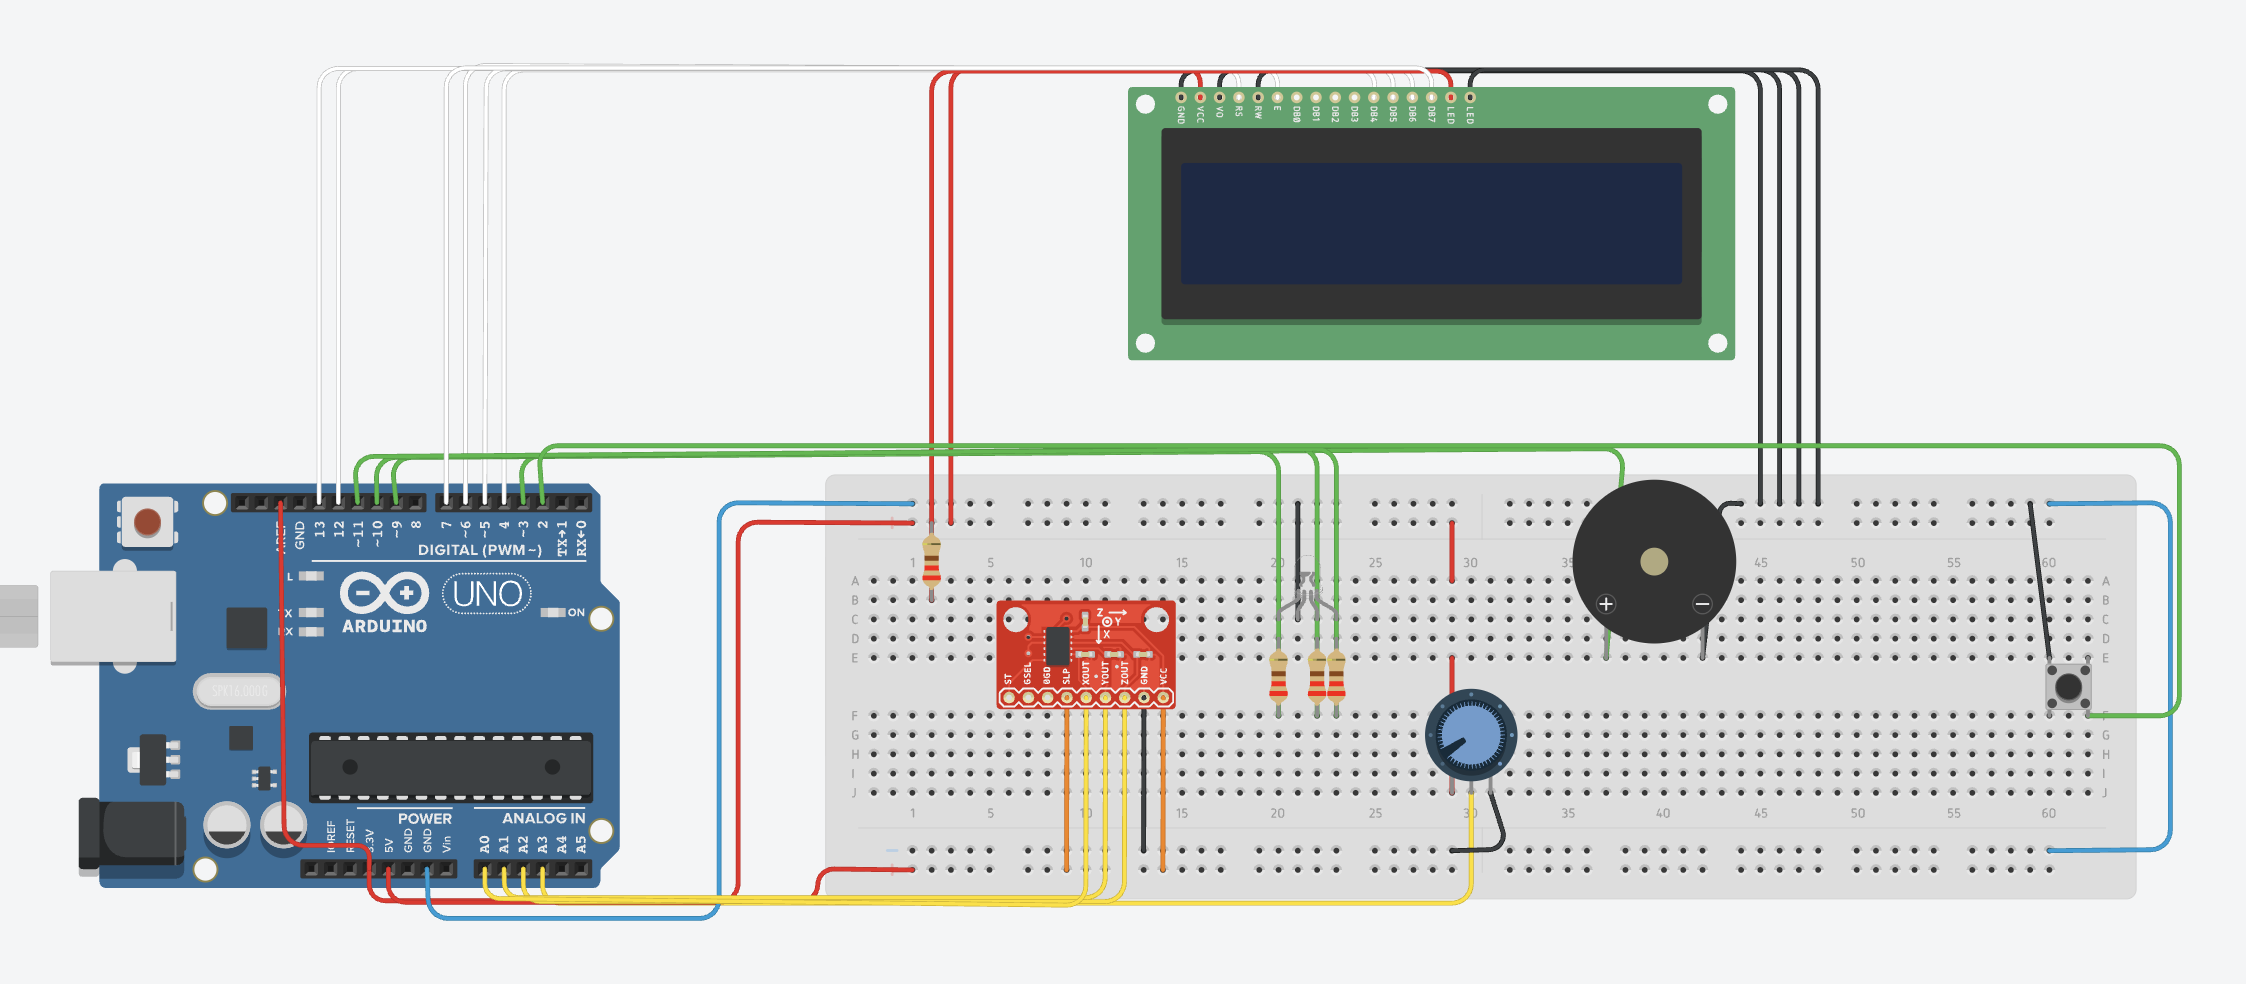
\includegraphics[width=0.8\textwidth]{figuras/circuito_tinkercad.png}
    \caption{Circuito do SMN-Q montado na plataforma Tinkercad.}
    \label{fig:circuito}
\end{figure}

\subsection{\esp Algoritmo de detecção}

A cada 100 ms o sistema lê os três eixos do acelerômetro e calcula a magnitude resultante (Equação \ref{eq:magnitude}). Sobre o valor calculado é aplicado um filtro de média móvel de 10 amostras, que suaviza ruídos do sensor sem afetar eventos de queda --- que duram várias amostras consecutivas.

\begin{equation}
\label{eq:magnitude}
Norm(x, y, z) = \sqrt{x^{2} + y^{2} + z^{2}}
\end{equation}

A magnitude filtrada é comparada com um valor de referência (\textit{base}), obtido na calibração inicial executada durante 5 segundos no \textit{boot}, com o usuário em repouso. Esse procedimento elimina variações de fabricação do sensor e da posição inicial do dispositivo.

A literatura tradicional sugere limiares fixos para identificar a queda livre (abaixo de 0,6g) e o impacto (acima de 2,5g) em sequência. Como o ambiente Tinkercad tem limitações para reproduzir esse tipo de movimento, adotamos uma abordagem simplificada baseada na variação absoluta da magnitude em relação à \textit{base}. Quando essa diferença ultrapassa o limite definido pelo potenciômetro, o sistema entra em estado de alerta. O potenciômetro oferece três níveis de sensibilidade: alta (0,50g), média (1,00g) e baixa (1,50g), permitindo ajustar o dispositivo ao perfil do idoso --- mais sensível para uma pessoa frágil, menos sensível para alguém ativo.

\subsection{\esp Rotina de teste}

Foi implementada uma rotina acionada pela tecla \verb|t| no Monitor Serial. Ela mostra as leituras de todas as entradas, aciona cada saída em sequência (LED nas quatro cores, buzzer, LCD) e retorna ao estado normal. Serve para validar rapidamente se o circuito está respondendo corretamente.

\section{\esp Resultados}

O protótipo atendeu aos requisitos do projeto: três tipos de entrada, três tipos de saída, filtragem com média móvel no sensor principal, calibração via potenciômetro e código organizado em funções. O Algoritmo \ref{alg:ciclo-alerta} mostra a sequência executada quando o sistema detecta uma possível queda. A janela de 15 segundos para cancelamento permite que o usuário interrompa o alarme em caso de falso positivo --- por exemplo, ao tropeçar e se recuperar sozinho.

\begin{center}
\begin{minipage}[ht]{13cm}
\begin{algorithm}[H]
  \footnotesize
  \caption{Ciclo de Alerta e Emergência}
  \label{alg:ciclo-alerta}
  \begin{algorithmic}[1]
    \STATE \textbf{Entrada:} Evento de queda detectado pelo acelerômetro
    \STATE \textbf{Saída:} Notificação ao cuidador ou cancelamento
    \STATE Aciona LED amarelo, buzzer de alerta e exibe ``Possível queda detectada'' no LCD
    \STATE Inicia contagem regressiva de 15 segundos
    \FOR{$t = 15$ \TO $1$}
        \STATE Exibe $t$ no LCD
        \IF{botão pressionado}
            \STATE Cancela alarme e retorna ao estado normal
            \STATE \textbf{Retorna}
        \ENDIF
        \STATE Aguarda 1 segundo
    \ENDFOR
    \STATE Aciona LED vermelho, buzzer forte e exibe ``EMERGÊNCIA!'' no LCD
    \STATE Envia notificação push ao cuidador (simulada via Serial Monitor)
  \end{algorithmic}
\end{algorithm}
\end{minipage}
\end{center}

O LED RGB sinaliza visualmente cada estado do sistema: verde para monitoramento normal, amarelo durante o alerta e vermelho na emergência confirmada. Essa codificação por cores facilita o entendimento rápido do que está acontecendo.

\begin{figure}[H]
    \centering
    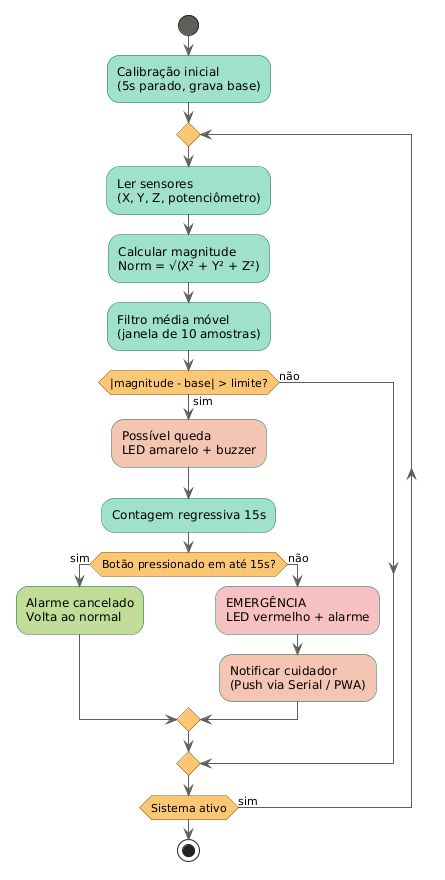
\includegraphics[width=0.7\textwidth]{figuras/fluxograma_sistema.png}
    \caption{Fluxograma do funcionamento do sistema SMN-Q.}
    \label{fig:fluxograma}
\end{figure}

Para facilitar a demonstração do funcionamento no Tinkercad, foi implementado o comando \verb|q| no Monitor Serial, que dispara diretamente o ciclo de alerta sem precisar manipular o acelerômetro na simulação.

\section{\esp Conclusão}

O SMN-Q foi implementado no Tinkercad e cumpriu todos os requisitos técnicos do projeto. O algoritmo baseado em magnitude resultante com filtro de média móvel funcionou de forma estável, e a janela de cancelamento de 15 segundos ajuda a evitar que falsos alarmes incomodem o usuário.

A implementação física do sistema é viável e acessível. Substituindo o Arduino UNO por um ESP32-C3 Super Mini, que já tem Wi-Fi integrado, e o MMA7361 por um MPU6050, o custo total estimado fica entre R\$ 200,00 e R\$ 280,00 --- muito abaixo das mensalidades das soluções comerciais. A notificação ao cuidador poderia ser feita por um Progressive Web App (PWA) com Firebase Cloud Messaging, chegando direto no celular como push notification.

Como melhorias futuras, três caminhos parecem promissores: implementar o algoritmo de quatro fases proposto por \citeonline{vieira2019}, que diferencia melhor as etapas da queda; adicionar a distinção entre quedas bruscas e suaves conforme \citeonline{cabral2022}, capturando também escorregões lentos; e desenvolver a calibração adaptativa personalizada proposta por \citeonline{ren2015}, em que o sistema aprende o padrão de cada usuário ao longo do tempo.